
% Default to the notebook output style

    


% Inherit from the specified cell style.




    
\documentclass[11pt]{article}

    
    
    \usepackage[T1]{fontenc}
    % Nicer default font (+ math font) than Computer Modern for most use cases
    \usepackage{mathpazo}

    % Basic figure setup, for now with no caption control since it's done
    % automatically by Pandoc (which extracts ![](path) syntax from Markdown).
    \usepackage{graphicx}
    % We will generate all images so they have a width \maxwidth. This means
    % that they will get their normal width if they fit onto the page, but
    % are scaled down if they would overflow the margins.
    \makeatletter
    \def\maxwidth{\ifdim\Gin@nat@width>\linewidth\linewidth
    \else\Gin@nat@width\fi}
    \makeatother
    \let\Oldincludegraphics\includegraphics
    % Set max figure width to be 80% of text width, for now hardcoded.
    %\renewcommand{\includegraphics}[1]{\Oldincludegraphics[width=.8\maxwidth]{#1}}
    % Ensure that by default, figures have no caption (until we provide a
    % proper Figure object with a Caption API and a way to capture that
    % in the conversion process - todo).
    \usepackage{caption}
    \DeclareCaptionLabelFormat{nolabel}{}
    \captionsetup{labelformat=nolabel}

    \usepackage{adjustbox} % Used to constrain images to a maximum size 
    \usepackage{xcolor} % Allow colors to be defined
    \usepackage{enumerate} % Needed for markdown enumerations to work
    \usepackage{geometry} % Used to adjust the document margins
    \usepackage{amsmath} % Equations
    \usepackage{amssymb} % Equations
    \usepackage{textcomp} % defines textquotesingle
    % Hack from http://tex.stackexchange.com/a/47451/13684:
    \AtBeginDocument{%
        \def\PYZsq{\textquotesingle}% Upright quotes in Pygmentized code
    }
    \usepackage{upquote} % Upright quotes for verbatim code
    \usepackage{eurosym} % defines \euro
    \usepackage[mathletters]{ucs} % Extended unicode (utf-8) support
    \usepackage[utf8x]{inputenc} % Allow utf-8 characters in the tex document
    \usepackage{fancyvrb} % verbatim replacement that allows latex
    \usepackage{grffile} % extends the file name processing of package graphics 
                         % to support a larger range 
    % The hyperref package gives us a pdf with properly built
    % internal navigation ('pdf bookmarks' for the table of contents,
    % internal cross-reference links, web links for URLs, etc.)
    \usepackage{hyperref}
    \usepackage{longtable} % longtable support required by pandoc >1.10
    \usepackage{booktabs}  % table support for pandoc > 1.12.2
    \usepackage[inline]{enumitem} % IRkernel/repr support (it uses the enumerate* environment)
    \usepackage[normalem]{ulem} % ulem is needed to support strikethroughs (\sout)
                                % normalem makes italics be italics, not underlines
    \usepackage{mathrsfs}
    

    
    
    % Colors for the hyperref package
    \definecolor{urlcolor}{rgb}{0,.145,.698}
    \definecolor{linkcolor}{rgb}{.71,0.21,0.01}
    \definecolor{citecolor}{rgb}{.12,.54,.11}

    % ANSI colors
    \definecolor{ansi-black}{HTML}{3E424D}
    \definecolor{ansi-black-intense}{HTML}{282C36}
    \definecolor{ansi-red}{HTML}{E75C58}
    \definecolor{ansi-red-intense}{HTML}{B22B31}
    \definecolor{ansi-green}{HTML}{00A250}
    \definecolor{ansi-green-intense}{HTML}{007427}
    \definecolor{ansi-yellow}{HTML}{DDB62B}
    \definecolor{ansi-yellow-intense}{HTML}{B27D12}
    \definecolor{ansi-blue}{HTML}{208FFB}
    \definecolor{ansi-blue-intense}{HTML}{0065CA}
    \definecolor{ansi-magenta}{HTML}{D160C4}
    \definecolor{ansi-magenta-intense}{HTML}{A03196}
    \definecolor{ansi-cyan}{HTML}{60C6C8}
    \definecolor{ansi-cyan-intense}{HTML}{258F8F}
    \definecolor{ansi-white}{HTML}{C5C1B4}
    \definecolor{ansi-white-intense}{HTML}{A1A6B2}
    \definecolor{ansi-default-inverse-fg}{HTML}{FFFFFF}
    \definecolor{ansi-default-inverse-bg}{HTML}{000000}

    % commands and environments needed by pandoc snippets
    % extracted from the output of `pandoc -s`
    \providecommand{\tightlist}{%
      \setlength{\itemsep}{0pt}\setlength{\parskip}{0pt}}
    \DefineVerbatimEnvironment{Highlighting}{Verbatim}{commandchars=\\\{\}}
    % Add ',fontsize=\small' for more characters per line
    \newenvironment{Shaded}{}{}
    \newcommand{\KeywordTok}[1]{\textcolor[rgb]{0.00,0.44,0.13}{\textbf{{#1}}}}
    \newcommand{\DataTypeTok}[1]{\textcolor[rgb]{0.56,0.13,0.00}{{#1}}}
    \newcommand{\DecValTok}[1]{\textcolor[rgb]{0.25,0.63,0.44}{{#1}}}
    \newcommand{\BaseNTok}[1]{\textcolor[rgb]{0.25,0.63,0.44}{{#1}}}
    \newcommand{\FloatTok}[1]{\textcolor[rgb]{0.25,0.63,0.44}{{#1}}}
    \newcommand{\CharTok}[1]{\textcolor[rgb]{0.25,0.44,0.63}{{#1}}}
    \newcommand{\StringTok}[1]{\textcolor[rgb]{0.25,0.44,0.63}{{#1}}}
    \newcommand{\CommentTok}[1]{\textcolor[rgb]{0.38,0.63,0.69}{\textit{{#1}}}}
    \newcommand{\OtherTok}[1]{\textcolor[rgb]{0.00,0.44,0.13}{{#1}}}
    \newcommand{\AlertTok}[1]{\textcolor[rgb]{1.00,0.00,0.00}{\textbf{{#1}}}}
    \newcommand{\FunctionTok}[1]{\textcolor[rgb]{0.02,0.16,0.49}{{#1}}}
    \newcommand{\RegionMarkerTok}[1]{{#1}}
    \newcommand{\ErrorTok}[1]{\textcolor[rgb]{1.00,0.00,0.00}{\textbf{{#1}}}}
    \newcommand{\NormalTok}[1]{{#1}}
    
    % Additional commands for more recent versions of Pandoc
    \newcommand{\ConstantTok}[1]{\textcolor[rgb]{0.53,0.00,0.00}{{#1}}}
    \newcommand{\SpecialCharTok}[1]{\textcolor[rgb]{0.25,0.44,0.63}{{#1}}}
    \newcommand{\VerbatimStringTok}[1]{\textcolor[rgb]{0.25,0.44,0.63}{{#1}}}
    \newcommand{\SpecialStringTok}[1]{\textcolor[rgb]{0.73,0.40,0.53}{{#1}}}
    \newcommand{\ImportTok}[1]{{#1}}
    \newcommand{\DocumentationTok}[1]{\textcolor[rgb]{0.73,0.13,0.13}{\textit{{#1}}}}
    \newcommand{\AnnotationTok}[1]{\textcolor[rgb]{0.38,0.63,0.69}{\textbf{\textit{{#1}}}}}
    \newcommand{\CommentVarTok}[1]{\textcolor[rgb]{0.38,0.63,0.69}{\textbf{\textit{{#1}}}}}
    \newcommand{\VariableTok}[1]{\textcolor[rgb]{0.10,0.09,0.49}{{#1}}}
    \newcommand{\ControlFlowTok}[1]{\textcolor[rgb]{0.00,0.44,0.13}{\textbf{{#1}}}}
    \newcommand{\OperatorTok}[1]{\textcolor[rgb]{0.40,0.40,0.40}{{#1}}}
    \newcommand{\BuiltInTok}[1]{{#1}}
    \newcommand{\ExtensionTok}[1]{{#1}}
    \newcommand{\PreprocessorTok}[1]{\textcolor[rgb]{0.74,0.48,0.00}{{#1}}}
    \newcommand{\AttributeTok}[1]{\textcolor[rgb]{0.49,0.56,0.16}{{#1}}}
    \newcommand{\InformationTok}[1]{\textcolor[rgb]{0.38,0.63,0.69}{\textbf{\textit{{#1}}}}}
    \newcommand{\WarningTok}[1]{\textcolor[rgb]{0.38,0.63,0.69}{\textbf{\textit{{#1}}}}}
    
    
    % Define a nice break command that doesn't care if a line doesn't already
    % exist.
    \def\br{\hspace*{\fill} \\* }
    % Math Jax compatibility definitions
    \def\gt{>}
    \def\lt{<}
    \let\Oldtex\TeX
    \let\Oldlatex\LaTeX
    \renewcommand{\TeX}{\textrm{\Oldtex}}
    \renewcommand{\LaTeX}{\textrm{\Oldlatex}}
    % Document parameters
    % Document title
    \title{Swaps and Bootstrapping - Practical Lesson 5}
    \author{Matteo Sani\\\href{mailto:matteosan1@gmail.com}{matteosan1@gmail.com}}
    
    
    
    

    % Pygments definitions
    
\makeatletter
\def\PY@reset{\let\PY@it=\relax \let\PY@bf=\relax%
    \let\PY@ul=\relax \let\PY@tc=\relax%
    \let\PY@bc=\relax \let\PY@ff=\relax}
\def\PY@tok#1{\csname PY@tok@#1\endcsname}
\def\PY@toks#1+{\ifx\relax#1\empty\else%
    \PY@tok{#1}\expandafter\PY@toks\fi}
\def\PY@do#1{\PY@bc{\PY@tc{\PY@ul{%
    \PY@it{\PY@bf{\PY@ff{#1}}}}}}}
\def\PY#1#2{\PY@reset\PY@toks#1+\relax+\PY@do{#2}}

\expandafter\def\csname PY@tok@w\endcsname{\def\PY@tc##1{\textcolor[rgb]{0.73,0.73,0.73}{##1}}}
\expandafter\def\csname PY@tok@c\endcsname{\let\PY@it=\textit\def\PY@tc##1{\textcolor[rgb]{0.25,0.50,0.50}{##1}}}
\expandafter\def\csname PY@tok@cp\endcsname{\def\PY@tc##1{\textcolor[rgb]{0.74,0.48,0.00}{##1}}}
\expandafter\def\csname PY@tok@k\endcsname{\let\PY@bf=\textbf\def\PY@tc##1{\textcolor[rgb]{0.00,0.50,0.00}{##1}}}
\expandafter\def\csname PY@tok@kp\endcsname{\def\PY@tc##1{\textcolor[rgb]{0.00,0.50,0.00}{##1}}}
\expandafter\def\csname PY@tok@kt\endcsname{\def\PY@tc##1{\textcolor[rgb]{0.69,0.00,0.25}{##1}}}
\expandafter\def\csname PY@tok@o\endcsname{\def\PY@tc##1{\textcolor[rgb]{0.40,0.40,0.40}{##1}}}
\expandafter\def\csname PY@tok@ow\endcsname{\let\PY@bf=\textbf\def\PY@tc##1{\textcolor[rgb]{0.67,0.13,1.00}{##1}}}
\expandafter\def\csname PY@tok@nb\endcsname{\def\PY@tc##1{\textcolor[rgb]{0.00,0.50,0.00}{##1}}}
\expandafter\def\csname PY@tok@nf\endcsname{\def\PY@tc##1{\textcolor[rgb]{0.00,0.00,1.00}{##1}}}
\expandafter\def\csname PY@tok@nc\endcsname{\let\PY@bf=\textbf\def\PY@tc##1{\textcolor[rgb]{0.00,0.00,1.00}{##1}}}
\expandafter\def\csname PY@tok@nn\endcsname{\let\PY@bf=\textbf\def\PY@tc##1{\textcolor[rgb]{0.00,0.00,1.00}{##1}}}
\expandafter\def\csname PY@tok@ne\endcsname{\let\PY@bf=\textbf\def\PY@tc##1{\textcolor[rgb]{0.82,0.25,0.23}{##1}}}
\expandafter\def\csname PY@tok@nv\endcsname{\def\PY@tc##1{\textcolor[rgb]{0.10,0.09,0.49}{##1}}}
\expandafter\def\csname PY@tok@no\endcsname{\def\PY@tc##1{\textcolor[rgb]{0.53,0.00,0.00}{##1}}}
\expandafter\def\csname PY@tok@nl\endcsname{\def\PY@tc##1{\textcolor[rgb]{0.63,0.63,0.00}{##1}}}
\expandafter\def\csname PY@tok@ni\endcsname{\let\PY@bf=\textbf\def\PY@tc##1{\textcolor[rgb]{0.60,0.60,0.60}{##1}}}
\expandafter\def\csname PY@tok@na\endcsname{\def\PY@tc##1{\textcolor[rgb]{0.49,0.56,0.16}{##1}}}
\expandafter\def\csname PY@tok@nt\endcsname{\let\PY@bf=\textbf\def\PY@tc##1{\textcolor[rgb]{0.00,0.50,0.00}{##1}}}
\expandafter\def\csname PY@tok@nd\endcsname{\def\PY@tc##1{\textcolor[rgb]{0.67,0.13,1.00}{##1}}}
\expandafter\def\csname PY@tok@s\endcsname{\def\PY@tc##1{\textcolor[rgb]{0.73,0.13,0.13}{##1}}}
\expandafter\def\csname PY@tok@sd\endcsname{\let\PY@it=\textit\def\PY@tc##1{\textcolor[rgb]{0.73,0.13,0.13}{##1}}}
\expandafter\def\csname PY@tok@si\endcsname{\let\PY@bf=\textbf\def\PY@tc##1{\textcolor[rgb]{0.73,0.40,0.53}{##1}}}
\expandafter\def\csname PY@tok@se\endcsname{\let\PY@bf=\textbf\def\PY@tc##1{\textcolor[rgb]{0.73,0.40,0.13}{##1}}}
\expandafter\def\csname PY@tok@sr\endcsname{\def\PY@tc##1{\textcolor[rgb]{0.73,0.40,0.53}{##1}}}
\expandafter\def\csname PY@tok@ss\endcsname{\def\PY@tc##1{\textcolor[rgb]{0.10,0.09,0.49}{##1}}}
\expandafter\def\csname PY@tok@sx\endcsname{\def\PY@tc##1{\textcolor[rgb]{0.00,0.50,0.00}{##1}}}
\expandafter\def\csname PY@tok@m\endcsname{\def\PY@tc##1{\textcolor[rgb]{0.40,0.40,0.40}{##1}}}
\expandafter\def\csname PY@tok@gh\endcsname{\let\PY@bf=\textbf\def\PY@tc##1{\textcolor[rgb]{0.00,0.00,0.50}{##1}}}
\expandafter\def\csname PY@tok@gu\endcsname{\let\PY@bf=\textbf\def\PY@tc##1{\textcolor[rgb]{0.50,0.00,0.50}{##1}}}
\expandafter\def\csname PY@tok@gd\endcsname{\def\PY@tc##1{\textcolor[rgb]{0.63,0.00,0.00}{##1}}}
\expandafter\def\csname PY@tok@gi\endcsname{\def\PY@tc##1{\textcolor[rgb]{0.00,0.63,0.00}{##1}}}
\expandafter\def\csname PY@tok@gr\endcsname{\def\PY@tc##1{\textcolor[rgb]{1.00,0.00,0.00}{##1}}}
\expandafter\def\csname PY@tok@ge\endcsname{\let\PY@it=\textit}
\expandafter\def\csname PY@tok@gs\endcsname{\let\PY@bf=\textbf}
\expandafter\def\csname PY@tok@gp\endcsname{\let\PY@bf=\textbf\def\PY@tc##1{\textcolor[rgb]{0.00,0.00,0.50}{##1}}}
\expandafter\def\csname PY@tok@go\endcsname{\def\PY@tc##1{\textcolor[rgb]{0.53,0.53,0.53}{##1}}}
\expandafter\def\csname PY@tok@gt\endcsname{\def\PY@tc##1{\textcolor[rgb]{0.00,0.27,0.87}{##1}}}
\expandafter\def\csname PY@tok@err\endcsname{\def\PY@bc##1{\setlength{\fboxsep}{0pt}\fcolorbox[rgb]{1.00,0.00,0.00}{1,1,1}{\strut ##1}}}
\expandafter\def\csname PY@tok@kc\endcsname{\let\PY@bf=\textbf\def\PY@tc##1{\textcolor[rgb]{0.00,0.50,0.00}{##1}}}
\expandafter\def\csname PY@tok@kd\endcsname{\let\PY@bf=\textbf\def\PY@tc##1{\textcolor[rgb]{0.00,0.50,0.00}{##1}}}
\expandafter\def\csname PY@tok@kn\endcsname{\let\PY@bf=\textbf\def\PY@tc##1{\textcolor[rgb]{0.00,0.50,0.00}{##1}}}
\expandafter\def\csname PY@tok@kr\endcsname{\let\PY@bf=\textbf\def\PY@tc##1{\textcolor[rgb]{0.00,0.50,0.00}{##1}}}
\expandafter\def\csname PY@tok@bp\endcsname{\def\PY@tc##1{\textcolor[rgb]{0.00,0.50,0.00}{##1}}}
\expandafter\def\csname PY@tok@fm\endcsname{\def\PY@tc##1{\textcolor[rgb]{0.00,0.00,1.00}{##1}}}
\expandafter\def\csname PY@tok@vc\endcsname{\def\PY@tc##1{\textcolor[rgb]{0.10,0.09,0.49}{##1}}}
\expandafter\def\csname PY@tok@vg\endcsname{\def\PY@tc##1{\textcolor[rgb]{0.10,0.09,0.49}{##1}}}
\expandafter\def\csname PY@tok@vi\endcsname{\def\PY@tc##1{\textcolor[rgb]{0.10,0.09,0.49}{##1}}}
\expandafter\def\csname PY@tok@vm\endcsname{\def\PY@tc##1{\textcolor[rgb]{0.10,0.09,0.49}{##1}}}
\expandafter\def\csname PY@tok@sa\endcsname{\def\PY@tc##1{\textcolor[rgb]{0.73,0.13,0.13}{##1}}}
\expandafter\def\csname PY@tok@sb\endcsname{\def\PY@tc##1{\textcolor[rgb]{0.73,0.13,0.13}{##1}}}
\expandafter\def\csname PY@tok@sc\endcsname{\def\PY@tc##1{\textcolor[rgb]{0.73,0.13,0.13}{##1}}}
\expandafter\def\csname PY@tok@dl\endcsname{\def\PY@tc##1{\textcolor[rgb]{0.73,0.13,0.13}{##1}}}
\expandafter\def\csname PY@tok@s2\endcsname{\def\PY@tc##1{\textcolor[rgb]{0.73,0.13,0.13}{##1}}}
\expandafter\def\csname PY@tok@sh\endcsname{\def\PY@tc##1{\textcolor[rgb]{0.73,0.13,0.13}{##1}}}
\expandafter\def\csname PY@tok@s1\endcsname{\def\PY@tc##1{\textcolor[rgb]{0.73,0.13,0.13}{##1}}}
\expandafter\def\csname PY@tok@mb\endcsname{\def\PY@tc##1{\textcolor[rgb]{0.40,0.40,0.40}{##1}}}
\expandafter\def\csname PY@tok@mf\endcsname{\def\PY@tc##1{\textcolor[rgb]{0.40,0.40,0.40}{##1}}}
\expandafter\def\csname PY@tok@mh\endcsname{\def\PY@tc##1{\textcolor[rgb]{0.40,0.40,0.40}{##1}}}
\expandafter\def\csname PY@tok@mi\endcsname{\def\PY@tc##1{\textcolor[rgb]{0.40,0.40,0.40}{##1}}}
\expandafter\def\csname PY@tok@il\endcsname{\def\PY@tc##1{\textcolor[rgb]{0.40,0.40,0.40}{##1}}}
\expandafter\def\csname PY@tok@mo\endcsname{\def\PY@tc##1{\textcolor[rgb]{0.40,0.40,0.40}{##1}}}
\expandafter\def\csname PY@tok@ch\endcsname{\let\PY@it=\textit\def\PY@tc##1{\textcolor[rgb]{0.25,0.50,0.50}{##1}}}
\expandafter\def\csname PY@tok@cm\endcsname{\let\PY@it=\textit\def\PY@tc##1{\textcolor[rgb]{0.25,0.50,0.50}{##1}}}
\expandafter\def\csname PY@tok@cpf\endcsname{\let\PY@it=\textit\def\PY@tc##1{\textcolor[rgb]{0.25,0.50,0.50}{##1}}}
\expandafter\def\csname PY@tok@c1\endcsname{\let\PY@it=\textit\def\PY@tc##1{\textcolor[rgb]{0.25,0.50,0.50}{##1}}}
\expandafter\def\csname PY@tok@cs\endcsname{\let\PY@it=\textit\def\PY@tc##1{\textcolor[rgb]{0.25,0.50,0.50}{##1}}}

\def\PYZbs{\char`\\}
\def\PYZus{\char`\_}
\def\PYZob{\char`\{}
\def\PYZcb{\char`\}}
\def\PYZca{\char`\^}
\def\PYZam{\char`\&}
\def\PYZlt{\char`\<}
\def\PYZgt{\char`\>}
\def\PYZsh{\char`\#}
\def\PYZpc{\char`\%}
\def\PYZdl{\char`\$}
\def\PYZhy{\char`\-}
\def\PYZsq{\char`\'}
\def\PYZdq{\char`\"}
\def\PYZti{\char`\~}
% for compatibility with earlier versions
\def\PYZat{@}
\def\PYZlb{[}
\def\PYZrb{]}
\makeatother


    % Exact colors from NB
    \definecolor{incolor}{rgb}{0.0, 0.0, 0.5}
    \definecolor{outcolor}{rgb}{0.545, 0.0, 0.0}



    
    % Prevent overflowing lines due to hard-to-break entities
    \sloppy 
    % Setup hyperref package
    \hypersetup{
      breaklinks=true,  % so long urls are correctly broken across lines
      colorlinks=true,
      urlcolor=urlcolor,
      linkcolor=linkcolor,
      citecolor=citecolor,
      }
    % Slightly bigger margins than the latex defaults
    
    \geometry{verbose,tmargin=1in,bmargin=1in,lmargin=1in,rmargin=1in}
    
    

    \begin{document}
    
    
    \maketitle
    
    

    
    \hypertarget{swaps-and-bootstrapping---practical-lesson-5}{%
\section{Swaps and Bootstrapping}\label{swaps-and-bootstrapping---practical-lesson-5}}

\hypertarget{recap}{%
\subsection{Recap}\label{recap}}

\begin{itemize}
\tightlist
\item
  basic Python (mostly not related directly to finance)
\item
  how to implement a discount factor interpolation function
\item
  wrapping up functionality in classes in order to work with multiple
  data sets more easily
\item
  libor forward rate calculator
\end{itemize}

\hypertarget{todays-lesson}{%
\subsection{Today's lesson}\label{todays-lesson}}

We're going to look at:

\begin{itemize}
\tightlist
\item
  modules, and start building up our library of finance-related
  functionality;
\item
  implementing an Overnight Index Swap class for calculating the NPV of
  an OIS;
\item
  bootstrapping technique to derive discount curve.
\end{itemize}

\hypertarget{modules-again}{%
\subsection{Modules (again)}\label{modules-again}}

An interactive session (e.g notebook or interactive shell) is great for
quick testing and exploratory use, but once you have some code
(i.e.~functions or classes) which you'd like to reuse often, rather than
copy/pasting it every time you need it, you can save it in a .py file
and use it from your session (aka you can create your own library).
These work just like the modules we have been importing up to now,
except they're written by us\ldots{}

Today we're going to start writing a module called \textbf{finmarkets},
and over the course of the remaining lessons we'll add functionality
related to the theory lessons \textbf{(consider that you will be asked
to use as much as possible this module for your final project !).}

According to your preferred way of working there are different
instructions to write a module:

\begin{itemize}
\tightlist
\item
  take a look at \href{https://www.youtube.com/watch?v=AqCl65wxikw}{this video} for an example of how
  using your own module is done for \emph{Jupyter notebook};
\item
  if you prefer to work with \emph{repl.it} instead please look at 
  \href{https://repl.it/@MatteoSani/finmarkets}{this skeleton of project}
  which has a finmarkets module example.
\end{itemize}

So to start our financial module let's create a new file called
\texttt{finmarkets.py} and copy the \texttt{DiscountCurve} class you
have written last time into it. As for any other module we will be able
to import it and use its classes and functions. Let's try with an
example:

    \begin{Verbatim}[commandchars=\\\{\}]
{\color{incolor}In [{\color{incolor}1}]:} \PY{k+kn}{from} \PY{n+nn}{datetime} \PY{k}{import} \PY{n}{date}
        \PY{k+kn}{from} \PY{n+nn}{finmarkets} \PY{k}{import} \PY{n}{DiscountCurve}
        
        \PY{n}{curve} \PY{o}{=} \PY{n}{DiscountCurve}\PY{p}{(}\PY{n}{date}\PY{p}{(}\PY{l+m+mi}{2020}\PY{p}{,} \PY{l+m+mi}{1}\PY{p}{,} \PY{l+m+mi}{1}\PY{p}{)}\PY{p}{,}
                              \PY{p}{[}\PY{n}{date}\PY{p}{(}\PY{l+m+mi}{2020}\PY{p}{,} \PY{l+m+mi}{1}\PY{p}{,} \PY{l+m+mi}{1}\PY{p}{)}\PY{p}{,} 
                               \PY{n}{date}\PY{p}{(}\PY{l+m+mi}{2021}\PY{p}{,} \PY{l+m+mi}{6}\PY{p}{,} \PY{l+m+mi}{1}\PY{p}{)}\PY{p}{,} 
                               \PY{n}{date}\PY{p}{(}\PY{l+m+mi}{2022}\PY{p}{,} \PY{l+m+mi}{1}\PY{p}{,} \PY{l+m+mi}{1}\PY{p}{)}\PY{p}{]}\PY{p}{,}
                              \PY{p}{[}\PY{l+m+mf}{1.0}\PY{p}{,} \PY{l+m+mf}{0.98}\PY{p}{,} \PY{l+m+mf}{0.82}\PY{p}{]}\PY{p}{)}
        \PY{n}{curve}\PY{o}{.}\PY{n}{df}\PY{p}{(}\PY{n}{date}\PY{p}{(}\PY{l+m+mi}{2020}\PY{p}{,} \PY{l+m+mi}{7}\PY{p}{,} \PY{l+m+mi}{1}\PY{p}{)}\PY{p}{)}
\end{Verbatim}

\begin{Verbatim}[commandchars=\\\{\}]
{\color{outcolor}Out[{\color{outcolor}1}]:} 0.9929132520645648
\end{Verbatim}
            
    \hypertarget{overnight-index-swap}{%
\section{Overnight Index Swap}\label{overnight-index-swap}}

Overnight Index Swaps (OIS) are products which pay a floating coupon,
determined by overnight rate fixings over the reference periods, against
a fixed coupon. Interest rate swaps are usually used to mitigate the
risks of fluctuations of varying interest rates, or to benefit from
lower interest rates. We will always look at these products from the
point of view of the \textbf{receiver of the floating leg}. By
definition an OIS is defined by:

\begin{itemize}
\tightlist
\item
  a notional amount \(N\)
\item
  a start date \(d_0\)
\item
  a sequence of payment dates \(d_1,...,d_n\)
\item
  a fixed rate \(K\)
\end{itemize}

(n.b.~for simplicity we're assuming that the fixed and floating legs
have the same notional and payment dates, although this is not
necessarily always the case in practice).

At each payment date, the floating leg pays a cash flow determined as
follows:

\[f_{\mathrm{float},~i} = N \Bigg\{\prod_{d=d_{i-1}}^{d=d_i-1}\Big(1+r_{o/n}(d)\cdot\frac{1}{360}\Big) -1 \Bigg\}\]

(This formula is valid for an EONIA swap, i.e.~for OIS swaps in EUR,
other currencies might have different conventions. The \(\frac{1}{360}\)
fraction appears because EONIA rates are quoted using the ACT/360
daycount convention and here we're making the simplifying assumption of
ignoring weekends and holidays, so we assume that each overnight rate is
valid for only one day.)

The sum of the discounted expected values of these cash flows is

\[\mathrm{NPV}_{\mathrm{float}} = \sum_{i=1}^{n}D(d_i)\mathbb{E}[f_{\mathrm{float},~i}]\]

where \(D(d)\) is the discount factor with expiry \(d\). On the other
hand, by definition (remember practical lesson 4 with forward rates), we
also have the following relationship

\[\mathbb{E}[f_{\mathrm{float},~i}] = N\cdot\Big(\frac{D_{ois}(d_{i-1})}{D_{ois}(d_{i})} - 1\Big) \]

hence

\[\mathrm{NPV}_{\mathrm{float}} = N\cdot \sum_{i=1}^{n}D(d_i) \Big(\frac{D_{ois}(d_{i-1})}{D_{ois}(d_{i})} - 1\Big) \]

where \(D_{ois}(d)\) is the discount factor implied by OIS prices (we
will see it better later).

The correct curve to use for discounting the flows of a collateralized
contract, like OIS, is the one associated with the collateral. Since OIS
contracts are collateralized with cash, and cash accrues daily interes
at the overnight rate, the OIS curve is itself the correct curve with
which to discount the flows of an OIS contract !

In summary, \(D = D_{ois}\) so the NPV simplifies to

\begin{equation}
  \begin{split}
    \mathrm{NPV}_{\mathrm{float}} & = N\cdot\sum_{i=1}^{n}[D(d_{i-1}) - D(d_i)] =  \\
    &= N\cdot[(D(d_{0}) - D(d_{1})) + (D(d_{1}) - D(d_{2})) + ... + (D(d_{n-1}) - D(d_{n}))]\\
    &= N \cdot [D(d_0) - D(d_n)]
  \end{split}
\end{equation}
Each cash flow of the fixed leg is equal to

\[f_{\mathrm{fix},~i}=N\cdot K\cdot \frac{d_i - d_{i-1}}{360}\]

so the NPV of the fixed leg is

\[\mathrm{NPV}_{\mathrm{fix}} = N\cdot K\cdot \sum_{i=1}^{n}D(d_{i})\frac{d_i - d_{i-1}}{360}\]

\textbf{Ultimately the aim will be to take a series of OIS quotations,
and determine the discount factors implied by their prices.} To do this
we'll build a pricing \texttt{class}, which takes discount curve as the
input and produces the net present value (NPV) of the OIS as the output.
Then we'll put this function inside a numerical optimizer to invert the
process to determine the implied discount factors from their prices
(market quotes).

    \begin{Verbatim}[commandchars=\\\{\}]
{\color{incolor}In [{\color{incolor}2}]:} \PY{k}{class} \PY{n+nc}{OvernightIndexSwap}\PY{p}{:}
        
            \PY{c+c1}{\PYZsh{} this method is called to build the instance,}
            \PY{c+c1}{\PYZsh{} we take some data arguments and save them as}
            \PY{c+c1}{\PYZsh{} attributes of self }
            \PY{c+c1}{\PYZsh{} n.b.: payment\PYZus{}dates should be a list of dates,}
            \PY{c+c1}{\PYZsh{} including the start date as the first element}
            \PY{k}{def} \PY{n+nf}{\PYZus{}\PYZus{}init\PYZus{}\PYZus{}}\PY{p}{(}\PY{n+nb+bp}{self}\PY{p}{,} \PY{n}{notional}\PY{p}{,} \PY{n}{payment\PYZus{}dates}\PY{p}{,} \PY{n}{fixed\PYZus{}rate}\PY{p}{)}\PY{p}{:}
                \PY{n+nb+bp}{self}\PY{o}{.}\PY{n}{notional} \PY{o}{=} \PY{n}{notional}
                \PY{n+nb+bp}{self}\PY{o}{.}\PY{n}{payment\PYZus{}dates} \PY{o}{=} \PY{n}{payment\PYZus{}dates}
                \PY{n+nb+bp}{self}\PY{o}{.}\PY{n}{fixed\PYZus{}rate} \PY{o}{=} \PY{n}{fixed\PYZus{}rate}
                
            \PY{c+c1}{\PYZsh{} this method takes a discount curve and calculates}
            \PY{c+c1}{\PYZsh{} the NPV of the floating leg using that curve}
            \PY{k}{def} \PY{n+nf}{npv\PYZus{}floating\PYZus{}leg}\PY{p}{(}\PY{n+nb+bp}{self}\PY{p}{,} \PY{n}{discount\PYZus{}curve}\PY{p}{)}\PY{p}{:}
                \PY{c+c1}{\PYZsh{} self.payment\PYZus{}date s[0] is the start date of the swap}
                \PY{c+c1}{\PYZsh{} self.payment\PYZus{}date s[-1] is the last payment date of the swap}
                \PY{k}{return} \PY{n+nb+bp}{self}\PY{o}{.}\PY{n}{notional} \PY{o}{*} \PY{p}{(}\PY{n}{discount\PYZus{}curve}\PY{o}{.}\PY{n}{df}\PY{p}{(}\PY{n+nb+bp}{self}\PY{o}{.}\PY{n}{payment\PYZus{}dates}\PY{p}{[}\PY{l+m+mi}{0}\PY{p}{]}\PY{p}{)} \PY{o}{\PYZhy{}} 
                                        \PY{n}{discount\PYZus{}curve}\PY{o}{.}\PY{n}{df}\PY{p}{(}\PY{n+nb+bp}{self}\PY{o}{.}\PY{n}{payment\PYZus{}dates}\PY{p}{[}\PY{o}{\PYZhy{}}\PY{l+m+mi}{1}\PY{p}{]}\PY{p}{)}\PY{p}{)}
            
            \PY{c+c1}{\PYZsh{} this method takes a discount curve and calculates the NPV}
            \PY{c+c1}{\PYZsh{} of the fixed leg using that curve}
            \PY{k}{def} \PY{n+nf}{npv\PYZus{}fixed\PYZus{}leg}\PY{p}{(}\PY{n+nb+bp}{self}\PY{p}{,} \PY{n}{discount\PYZus{}curve}\PY{p}{)}\PY{p}{:}
                \PY{n}{npv} \PY{o}{=} \PY{l+m+mi}{0}
                \PY{c+c1}{\PYZsh{} we loop from i=1 up to but not including the length of the date list}
                \PY{k}{for} \PY{n}{i} \PY{o+ow}{in} \PY{n+nb}{range}\PY{p}{(}\PY{l+m+mi}{1}\PY{p}{,} \PY{n+nb}{len}\PY{p}{(}\PY{n+nb+bp}{self}\PY{o}{.}\PY{n}{payment\PYZus{}dates}\PY{p}{)}\PY{p}{)}\PY{p}{:} 
                    \PY{c+c1}{\PYZsh{} we can do i-1, because the loop starts with i=1}
                    \PY{n}{start\PYZus{}date} \PY{o}{=} \PY{n+nb+bp}{self}\PY{o}{.}\PY{n}{payment\PYZus{}dates}\PY{p}{[}\PY{n}{i}\PY{o}{\PYZhy{}}\PY{l+m+mi}{1}\PY{p}{]} 
                    \PY{n}{end\PYZus{}date} \PY{o}{=} \PY{n+nb+bp}{self}\PY{o}{.}\PY{n}{payment\PYZus{}dates}\PY{p}{[}\PY{n}{i}\PY{p}{]}
                    \PY{n}{tau} \PY{o}{=} \PY{p}{(}\PY{n}{end\PYZus{}date} \PY{o}{\PYZhy{}} \PY{n}{start\PYZus{}date}\PY{p}{)}\PY{o}{.}\PY{n}{days} \PY{o}{/} \PY{l+m+mi}{360}
                    \PY{n}{df} \PY{o}{=} \PY{n}{discount\PYZus{}curve}\PY{o}{.}\PY{n}{df}\PY{p}{(}\PY{n}{end\PYZus{}date}\PY{p}{)}
                    \PY{n}{npv} \PY{o}{=} \PY{n}{npv} \PY{o}{+} \PY{n}{df} \PY{o}{*} \PY{n}{tau}
                \PY{k}{return} \PY{n+nb+bp}{self}\PY{o}{.}\PY{n}{notional} \PY{o}{*} \PY{n+nb+bp}{self}\PY{o}{.}\PY{n}{fixed\PYZus{}rate} \PY{o}{*} \PY{n}{npv}
            
            \PY{c+c1}{\PYZsh{} this method calculates the NPV of the OIS swap}
            \PY{c+c1}{\PYZsh{} n.b.: inside this method we call the other two }
            \PY{c+c1}{\PYZsh{} methods of the class on the same instance \PYZsq{}self\PYZsq{},}
            \PY{c+c1}{\PYZsh{} using self.npv\PYZus{}XXX\PYZus{}leg(...), and we pass the }
            \PY{c+c1}{\PYZsh{} discount\PYZus{}curve we received as an argument}
            \PY{k}{def} \PY{n+nf}{npv}\PY{p}{(}\PY{n+nb+bp}{self}\PY{p}{,} \PY{n}{discount\PYZus{}curve}\PY{p}{)}\PY{p}{:}
                \PY{n}{float\PYZus{}npv} \PY{o}{=} \PY{n+nb+bp}{self}\PY{o}{.}\PY{n}{npv\PYZus{}floating\PYZus{}leg}\PY{p}{(}\PY{n}{discount\PYZus{}curve}\PY{p}{)}
                \PY{n}{fixed\PYZus{}npv} \PY{o}{=} \PY{n+nb+bp}{self}\PY{o}{.}\PY{n}{npv\PYZus{}fixed\PYZus{}leg}\PY{p}{(}\PY{n}{discount\PYZus{}curve}\PY{p}{)}
                \PY{k}{return} \PY{n}{float\PYZus{}npv} \PY{o}{\PYZhy{}} \PY{n}{fixed\PYZus{}npv}
\end{Verbatim}

    \begin{Verbatim}[commandchars=\\\{\}]
{\color{incolor}In [{\color{incolor}3}]:} \PY{k+kn}{from} \PY{n+nn}{datetime} \PY{k}{import} \PY{n}{date}
        
        \PY{n}{ois} \PY{o}{=} \PY{n}{OvernightIndexSwap}\PY{p}{(}
            \PY{c+c1}{\PYZsh{} the notional, one million}
            \PY{l+m+mf}{1e6}\PY{p}{,}
            \PY{c+c1}{\PYZsh{} the list of product dates, }
            \PY{c+c1}{\PYZsh{} i.e. the start date then the payment dates}
            \PY{p}{[}\PY{n}{date}\PY{p}{(}\PY{l+m+mi}{2020}\PY{p}{,} \PY{l+m+mi}{1}\PY{p}{,} \PY{l+m+mi}{1}\PY{p}{)}\PY{p}{,} 
             \PY{n}{date}\PY{p}{(}\PY{l+m+mi}{2020}\PY{p}{,} \PY{l+m+mi}{4}\PY{p}{,} \PY{l+m+mi}{1}\PY{p}{)}\PY{p}{,} 
             \PY{n}{date}\PY{p}{(}\PY{l+m+mi}{2020}\PY{p}{,} \PY{l+m+mi}{7}\PY{p}{,} \PY{l+m+mi}{1}\PY{p}{)}\PY{p}{,} 
             \PY{n}{date}\PY{p}{(}\PY{l+m+mi}{2020}\PY{p}{,} \PY{l+m+mi}{10}\PY{p}{,} \PY{l+m+mi}{1}\PY{p}{)}\PY{p}{,}
             \PY{n}{date}\PY{p}{(}\PY{l+m+mi}{2021}\PY{p}{,} \PY{l+m+mi}{1}\PY{p}{,} \PY{l+m+mi}{1}\PY{p}{)}\PY{p}{]}\PY{p}{,}
            \PY{c+c1}{\PYZsh{} the fixed rate, 2.5\PYZpc{}}
            \PY{l+m+mf}{0.025}
        \PY{p}{)}
\end{Verbatim}

    We can now use the curve we have prepared at the beginning of the lesson
and that we stored in a variable called curve to check if the class is
working by evaluating the NPV of the OIS.

    \begin{Verbatim}[commandchars=\\\{\}]
{\color{incolor}In [{\color{incolor}4}]:} \PY{n}{ois}\PY{o}{.}\PY{n}{npv}\PY{p}{(}\PY{n}{curve}\PY{p}{)}
\end{Verbatim}

\begin{Verbatim}[commandchars=\\\{\}]
{\color{outcolor}Out[{\color{outcolor}4}]:} -10990.364227052869
\end{Verbatim}
            
    \hypertarget{bootstrapping}{%
\subsection{Bootstrapping}\label{bootstrapping}}

Now we're going to look at how extract a discount curve from OIS market
data, via a process called \emph{bootstrapping}. This is the ABC of
financial mathematics, since you almost always need a discount curve to
price any contract, especially if you're interested in its NPV. We're
going to concentrate on EONIA swaps in order to build an EUR discount
curve.

\hypertarget{getting-the-data}{%
\subsubsection{Getting the data}\label{getting-the-data}}

The first problem is actually getting the data (swap market quotes) from
somewhere, and this is not actually as simple as it sounds.

The issue is that the EONIA swap market is Over The Counter (OTC) and
it's not straightforward to access it. Unlike (some) listed futures,
where anyone with a retail brokerage account can view and apply realtime
prices, to trade in the EONIA swap market you have to be a financial
institution or at least a large company and have an agreement with a
broker which operates in the market. One of the main brokers in the OIS
market is ICAP.

Though there exist some electronic platform in which market participants
post bids and offers and other participants can apply them, in practice
a lot of trading is still done over ``voice'', i.e.~by phone or more
commonly over chat. For convenience, however, Bloomberg provides a
service which displays indicative realtime rates as provided by a
selection of relevant brokers. (\emph{n.b.~interest rate swap quotes
vary from standard price quotes of commonly traded instruments, they can
appear puzzling because the quotes are effectively interest rates})

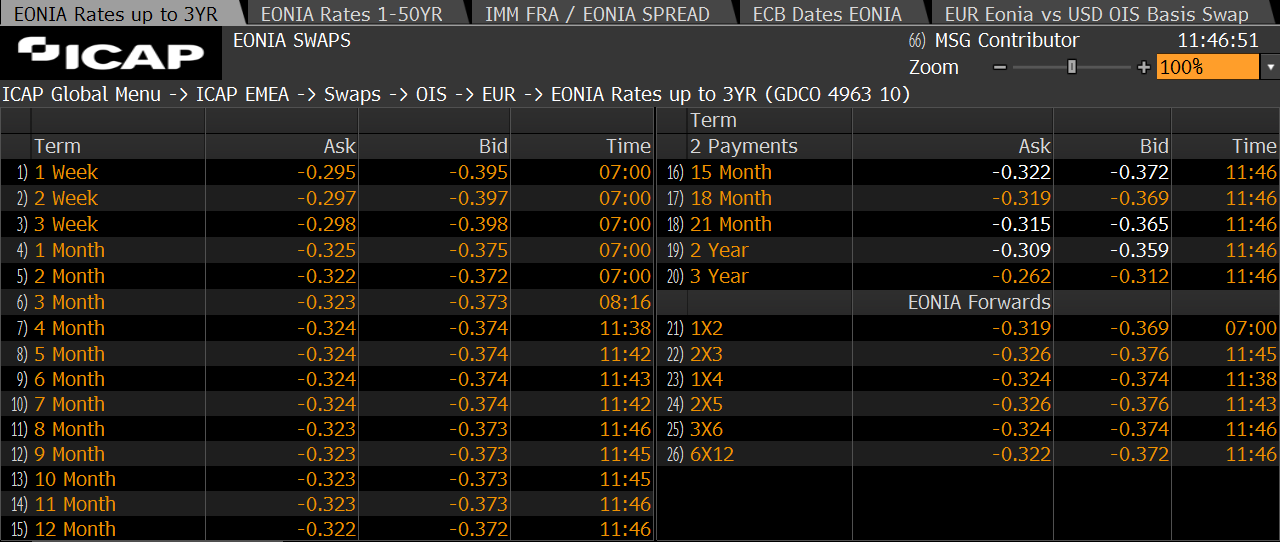
\includegraphics[width=\linewidth]{icap_3.png}

As part of our Quants duties we have set up an Excel spreadsheet which
acquires this data from Bloomberg in realtime. From this spreadsheet,
it's easy to export the data into a Python file - I have done this and
saved the data in a file (\texttt{ois\_data.py}).

We now use this dataset to derive a discount curve, let's check how it
looks like:

    \begin{Verbatim}[commandchars=\\\{\}]
{\color{incolor}In [{\color{incolor}5}]:} \PY{k+kn}{import} \PY{n+nn}{ois\PYZus{}data}
        \PY{n+nb}{print} \PY{p}{(}\PY{n+nb}{type}\PY{p}{(}\PY{n}{ois\PYZus{}data}\PY{o}{.}\PY{n}{quotes}\PY{p}{)}\PY{p}{)}
\end{Verbatim}

    \begin{Verbatim}[commandchars=\\\{\}]
<class 'list'>

    \end{Verbatim}

    \begin{Verbatim}[commandchars=\\\{\}]
{\color{incolor}In [{\color{incolor}6}]:} \PY{n}{ois\PYZus{}data}\PY{o}{.}\PY{n}{quotes}\PY{p}{[}\PY{l+m+mi}{0}\PY{p}{]}
\end{Verbatim}

\begin{Verbatim}[commandchars=\\\{\}]
{\color{outcolor}Out[{\color{outcolor}6}]:} \{'months': 1, 'rate': -0.35\}
\end{Verbatim}
            
    \begin{Verbatim}[commandchars=\\\{\}]
{\color{incolor}In [{\color{incolor}7}]:} \PY{n}{ois\PYZus{}data}\PY{o}{.}\PY{n}{quotes}\PY{p}{[}\PY{o}{\PYZhy{}}\PY{l+m+mi}{1}\PY{p}{]}
\end{Verbatim}

\begin{Verbatim}[commandchars=\\\{\}]
{\color{outcolor}Out[{\color{outcolor}7}]:} \{'months': 720, 'rate': 0.997\}
\end{Verbatim}
            
    \begin{Verbatim}[commandchars=\\\{\}]
{\color{incolor}In [{\color{incolor}8}]:} \PY{n}{ois\PYZus{}data}\PY{o}{.}\PY{n}{observation\PYZus{}date}
\end{Verbatim}

\begin{Verbatim}[commandchars=\\\{\}]
{\color{outcolor}Out[{\color{outcolor}8}]:} datetime.date(2019, 10, 23)
\end{Verbatim}
            
    \hypertarget{building-ois-instances}{%
\subsubsection{Building OIS instances}\label{building-ois-instances}}

Let's say we want to build a 15 months swap instance, we have to use
data contained in \texttt{ois\_data} file:

    \begin{Verbatim}[commandchars=\\\{\}]
{\color{incolor}In [{\color{incolor}9}]:} \PY{c+c1}{\PYZsh{} first check the 15 months rate}
        \PY{n}{ois\PYZus{}data}\PY{o}{.}\PY{n}{quotes}\PY{p}{[}\PY{l+m+mi}{12}\PY{p}{]}
\end{Verbatim}

\begin{Verbatim}[commandchars=\\\{\}]
{\color{outcolor}Out[{\color{outcolor}9}]:} \{'months': 15, 'rate': -0.35\}
\end{Verbatim}
            
    We can build the swap instance like this:

\begin{Shaded}
\begin{Highlighting}[]
\NormalTok{ois }\OperatorTok{=}\NormalTok{ OvernightIndexSwap(}\FloatTok{1e6}\NormalTok{,}
\NormalTok{                         [date(}\DecValTok{2019}\NormalTok{, }\DecValTok{10}\NormalTok{, }\DecValTok{23}\NormalTok{), }
\NormalTok{                          date(}\DecValTok{2020}\NormalTok{, }\DecValTok{10}\NormalTok{, }\DecValTok{23}\NormalTok{), }
\NormalTok{                          date(}\DecValTok{2020}\NormalTok{, }\DecValTok{1}\NormalTok{, }\DecValTok{23}\NormalTok{)],                        }
\NormalTok{                         ois_data.quotes[}\DecValTok{12}\NormalTok{][}\StringTok{'rate'}\NormalTok{]}\OperatorTok{*}\FloatTok{0.01} 
\NormalTok{                        )}
\CommentTok{# print the last payment date (15 months after obs date)}
\NormalTok{ois.payment_dates[}\OperatorTok{-}\DecValTok{1}\NormalTok{]}
\end{Highlighting}
\end{Shaded}

Clearly to use the \texttt{npv} method to calculate the OIS' NPV we need
a discount curve with which to evaluate it and here comes to hand the
bootstrapping technique !

    \hypertarget{exercise-5.1}{%
\subsubsection{Exercise 5.1}\label{exercise-5.1}}

Today and in the next lessons we're going to build lots of
\texttt{OvernightIndexSwap} objects, one for each market quote we have
(market quotes, as we have seen, consist of fixed strikes for 1M, 2M,
3M, \ldots{}, 12M, 15M, 18M, 2Y, 3Y, \ldots{}, 30Y and 40Y swaps).

It would be very boring to write a long list of payment dates for each
one of these, plus they'd need to be updated every day. Write a function
which given a start date and the number of months, returns a list of
dates of \textbf{annual} frequency starting from the start date and
ending after the specified number of months.

For example
\begin{itemize}
\item 2019-11-10 start date 12 months \(\rightarrow\) 2019-11-10, 2020-11-10
\item 2019-11-10 start date 24 months \(\rightarrow\) 2019-11-10, 2020-11-10, 2021-11-10
\end{itemize}

Note that if the number of months is not a multiple of 12, the last
period should simply be shorter than 12 months. For example

\begin{itemize}
\item 2019-11-10 start date 9 months \(\rightarrow\) 2019-11-10, 2020-08-10
\item 2019-11-10 start date 15 months \(\rightarrow\) 2019-11-10, 2020-11-10, 2021-02-10
\end{itemize}

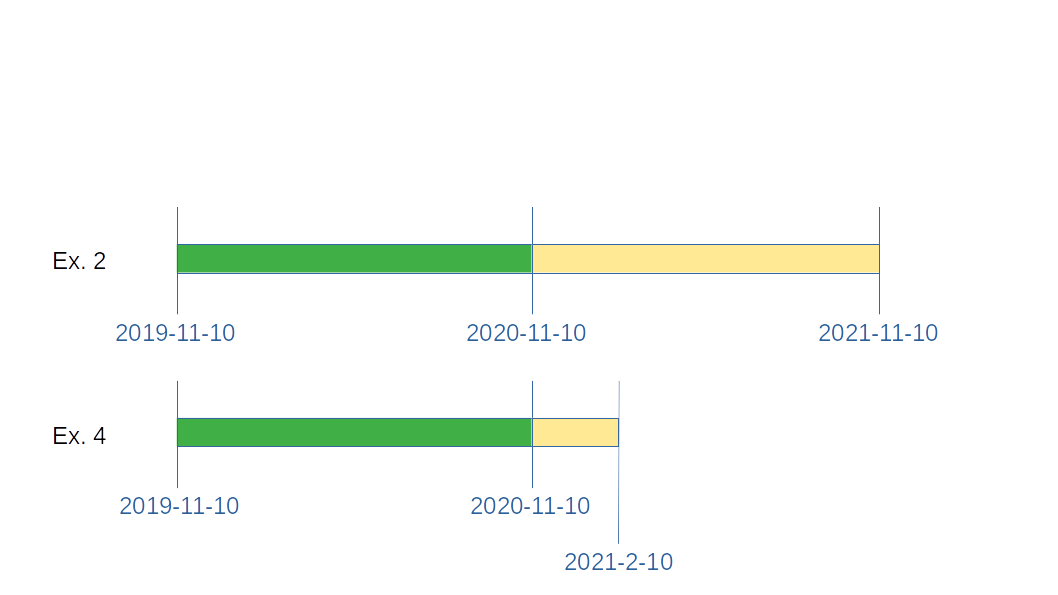
\includegraphics[width=\linewidth]{time_flow.png}

Here's some skeleton code to help you get started:

\begin{Shaded}
\begin{Highlighting}[]
\ImportTok{from}\NormalTok{ dateutil }\ImportTok{import}\NormalTok{ relativedelta}

\KeywordTok{def}\NormalTok{ generate_swap_dates(start_date, n_months):}
\NormalTok{    dates }\OperatorTok{=}\NormalTok{ []}
    \CommentTok{# your code here which adds all the relevant dates to the dates list}
    \ControlFlowTok{return}\NormalTok{ dates}
\end{Highlighting}
\end{Shaded}

\begin{Shaded}
\begin{Highlighting}[]
\CommentTok{# some tests to check if the function is working correctly}
\ImportTok{from}\NormalTok{ datetime }\ImportTok{import}\NormalTok{ date}

\ControlFlowTok{assert}\NormalTok{ generate_swap_dates(date(}\DecValTok{2019}\NormalTok{, }\DecValTok{11}\NormalTok{, }\DecValTok{10}\NormalTok{), }\DecValTok{12}\NormalTok{) }\OperatorTok{==}\NormalTok{ [date(}\DecValTok{2019}\NormalTok{, }\DecValTok{11}\NormalTok{, }\DecValTok{10}\NormalTok{), }
\NormalTok{                                                       date(}\DecValTok{2020}\NormalTok{, }\DecValTok{11}\NormalTok{, }\DecValTok{10}\NormalTok{)]}
\ControlFlowTok{assert}\NormalTok{ generate_swap_dates(date(}\DecValTok{2019}\NormalTok{, }\DecValTok{11}\NormalTok{, }\DecValTok{10}\NormalTok{), }\DecValTok{24}\NormalTok{) }\OperatorTok{==}\NormalTok{ [date(}\DecValTok{2019}\NormalTok{, }\DecValTok{11}\NormalTok{, }\DecValTok{10}\NormalTok{), }
\NormalTok{                                                       date(}\DecValTok{2020}\NormalTok{, }\DecValTok{11}\NormalTok{, }\DecValTok{10}\NormalTok{), }
\NormalTok{                                                       date(}\DecValTok{2021}\NormalTok{, }\DecValTok{11}\NormalTok{, }\DecValTok{10}\NormalTok{)]}

\ControlFlowTok{assert}\NormalTok{ generate_swap_dates(date(}\DecValTok{2019}\NormalTok{, }\DecValTok{11}\NormalTok{, }\DecValTok{10}\NormalTok{), }\DecValTok{9}\NormalTok{) }\OperatorTok{==}\NormalTok{ [date(}\DecValTok{2019}\NormalTok{, }\DecValTok{11}\NormalTok{, }\DecValTok{10}\NormalTok{), }
\NormalTok{                                                      date(}\DecValTok{2020}\NormalTok{, }\DecValTok{8}\NormalTok{, }\DecValTok{10}\NormalTok{)]}
\ControlFlowTok{assert}\NormalTok{ generate_swap_dates(date(}\DecValTok{2019}\NormalTok{, }\DecValTok{11}\NormalTok{, }\DecValTok{10}\NormalTok{), }\DecValTok{15}\NormalTok{) }\OperatorTok{==}\NormalTok{ [date(}\DecValTok{2019}\NormalTok{, }\DecValTok{11}\NormalTok{, }\DecValTok{10}\NormalTok{), }
\NormalTok{                                                       date(}\DecValTok{2020}\NormalTok{, }\DecValTok{11}\NormalTok{, }\DecValTok{10}\NormalTok{), }
\NormalTok{                                                       date(}\DecValTok{2021}\NormalTok{, }\DecValTok{2}\NormalTok{, }\DecValTok{10}\NormalTok{)]}
\end{Highlighting}
\end{Shaded}

    \hypertarget{the-bootstrapping-technique}{%
\subsubsection{The Bootstrapping
Technique}\label{the-bootstrapping-technique}}

In the next we are going to somehow reverse what we have previously done
(i.e.~we determined the OIS's NPV given a certain discount curve).

The general idea here is to get the discount curve such that it prices
correctly each OIS, or at least as well as possible, by minimizing the
sum of the square NPVs:

\[\mathrm{min}_{curve} \Big\{\sum_{i=1}^{n}\mathrm{NPV}(\mathrm{ois}_i, \mathrm{curve})^2\Big\}\]

A discount curve is characterized by pillar dates and the corresponding
discount factors. The description of the problem we have given above
does not, in theory, specifies any constraint on the pillar dates of the
discount curve. However, the pillar dates determine the number of
unknown variables (i.e.~the dimensionality \(n\) of the optimization
problem). A curve with \(n\) pillar dates has \(n\) discount factors
(note that the first discount factor with value date equal to the today
date, is constrained to 1). \textbf{In practice, therefore, it makes
sense to choose the pillar dates in such a way that there are exactly
the right number of degrees of freedom in the optimization to match
data.} So the natural choice is to choose the pillar dates of the
discount curve equal to the set of expiry dates of the swaps.

The reason for this is that each market quote will determine exactly one
\emph{free} discount factor which is not already determined by the other
market quotes - this can be seen by considering the mathematical
expression for calculating the fixed leg of the OIS swaps
(\(f_{\mathrm{fix},~i}=N\cdot K\cdot D(d_i)\cdot\frac{d_i - d_{i-1}}{360}\)),
and the way that the payment date schedules are constructed. Therefore,
once we've fixed \(\vec{d}\) to be a vector of pillar dates equal to the
expiry dates of the OIS swaps, and we use the notation \(\vec{x}\) to
represent the vector of pillar discount factors, then the problem
becomes:

\[\mathrm{min}_{\vec{x}} \Big\{\sum_{i=1}^{n}\mathrm{NPV}(\mathrm{ois}_i, \mathrm{curve(\vec{d}, \vec{x})})^2\Big\}\]

In practice this is an optmization problem (\textbf{to find the minimum
of the above expression as a function of \(\vec{x}\)}) so we can just
use one of the available numerical optimization routines.

So let's start by defining a set of OIS objects to cover all the
maturities defined by the market data we have collected in the
\texttt{ois\_data.py} file.

    \begin{Verbatim}[commandchars=\\\{\}]
{\color{incolor}In [{\color{incolor}10}]:} \PY{k+kn}{from} \PY{n+nn}{finmarkets} \PY{k}{import} \PY{n}{DiscountCurve}\PY{p}{,} \PY{n}{generate\PYZus{}swap\PYZus{}dates}
         \PY{k+kn}{import} \PY{n+nn}{ois\PYZus{}data\PYZus{}eric} \PY{k}{as} \PY{n+nn}{ois\PYZus{}data}
         
         \PY{n}{pillar\PYZus{}dates} \PY{o}{=} \PY{p}{[}\PY{n}{ois\PYZus{}data}\PY{o}{.}\PY{n}{observation\PYZus{}date}\PY{p}{]}
         
         \PY{n}{swaps} \PY{o}{=} \PY{p}{[}\PY{p}{]} \PY{c+c1}{\PYZsh{} container of the OIS objects}
         
         \PY{k}{for} \PY{n}{quote} \PY{o+ow}{in} \PY{n}{ois\PYZus{}data}\PY{o}{.}\PY{n}{quotes}\PY{p}{:}
             \PY{n}{swap} \PY{o}{=} \PY{n}{OvernightIndexSwap}\PY{p}{(}
                 \PY{c+c1}{\PYZsh{} notional \PYZhy{} doesn\PYZsq{}t really matter what we put here}
                 \PY{l+m+mf}{1e6}\PY{p}{,}
                 
                 \PY{c+c1}{\PYZsh{} payment dates}
                 \PY{n}{generate\PYZus{}swap\PYZus{}dates}\PY{p}{(}
                     \PY{n}{ois\PYZus{}data}\PY{o}{.}\PY{n}{observation\PYZus{}date}\PY{p}{,}
                     \PY{n}{quote}\PY{p}{[}\PY{l+s+s1}{\PYZsq{}}\PY{l+s+s1}{months}\PY{l+s+s1}{\PYZsq{}}\PY{p}{]}
                 \PY{p}{)}\PY{p}{,}
                 
                 \PY{c+c1}{\PYZsh{} the fixed rate (in the file is expressed in percent)}
                 \PY{l+m+mf}{0.01} \PY{o}{*} \PY{n}{quote}\PY{p}{[}\PY{l+s+s1}{\PYZsq{}}\PY{l+s+s1}{rate}\PY{l+s+s1}{\PYZsq{}}\PY{p}{]}
             \PY{p}{)}
             \PY{n}{swaps}\PY{o}{.}\PY{n}{append}\PY{p}{(}\PY{n}{swap}\PY{p}{)}
             \PY{n}{pillar\PYZus{}dates}\PY{o}{.}\PY{n}{append}\PY{p}{(}\PY{n}{swap}\PY{o}{.}\PY{n}{payment\PYZus{}dates}\PY{p}{[}\PY{o}{\PYZhy{}}\PY{l+m+mi}{1}\PY{p}{]}\PY{p}{)}
             
         \PY{n}{pillar\PYZus{}dates} \PY{o}{=} \PY{n+nb}{sorted}\PY{p}{(}\PY{n}{pillar\PYZus{}dates}\PY{p}{)}
         \PY{n}{n\PYZus{}df\PYZus{}vector} \PY{o}{=} \PY{n+nb}{len}\PY{p}{(}\PY{n}{pillar\PYZus{}dates}\PY{p}{)}
\end{Verbatim}

    \begin{Verbatim}[commandchars=\\\{\}]
{\color{incolor}In [{\color{incolor}11}]:} \PY{n+nb}{type}\PY{p}{(}\PY{n}{pillar\PYZus{}dates}\PY{p}{)}\PY{p}{,} \PY{n+nb}{len}\PY{p}{(}\PY{n}{pillar\PYZus{}dates}\PY{p}{)}\PY{p}{,} \PY{n}{pillar\PYZus{}dates}\PY{p}{[}\PY{l+m+mi}{0}\PY{p}{]}\PY{p}{,} \PY{n}{pillar\PYZus{}dates}\PY{p}{[}\PY{o}{\PYZhy{}}\PY{l+m+mi}{1}\PY{p}{]}
\end{Verbatim}

\begin{Verbatim}[commandchars=\\\{\}]
{\color{outcolor}Out[{\color{outcolor}11}]:} (list, 34, datetime.date(2016, 11, 23), datetime.date(2076, 11, 23))
\end{Verbatim}
            
    \hypertarget{how-does-the-minimization-algorithm-work}{%
\paragraph{How Does the Minimization Algorithm Work
?}\label{how-does-the-minimization-algorithm-work}}

\begin{itemize}
\item
  Define an \emph{objective function} i.e.~the function that is actually
  minimized to reach our goal. In our case we want to find the discount
  curve which minimize the sum of the squared NPVs (swap quotes are
  considered their fair-values);
\item
  set the intial value of the unknown parameters and their range of
  variability. We will set all the discount factors to 1 with a range of
  \([0.01, 100]\) (of course the first element of the list, today's
  discount factor will be set constant to 1);
\item
  the \emph{minimizer} will compute the objective function value;
\item
  then will move the parameter values in such a way to find a smaller
  value of the objective function (e.g.~\emph{following} the derivative
  w.r.t. each parameter);
\item
  the last two steps will be repeated until further variations of the x
  values won't change significantly the objective function (i.e.~we have
  found a minimum of the function so the minimization process is
  completed !).
\end{itemize}

    \begin{Verbatim}[commandchars=\\\{\}]
{\color{incolor}In [{\color{incolor}12}]:} \PY{k}{def} \PY{n+nf}{objective\PYZus{}function}\PY{p}{(}\PY{n}{x}\PY{p}{)}\PY{p}{:}
             
             \PY{n}{curve} \PY{o}{=} \PY{n}{DiscountCurve}\PY{p}{(}       
                 \PY{n}{ois\PYZus{}data}\PY{o}{.}\PY{n}{observation\PYZus{}date}\PY{p}{,}
                 \PY{n}{pillar\PYZus{}dates}\PY{p}{,}
                 \PY{n}{x}
             \PY{p}{)}
             
             \PY{n}{sum\PYZus{}sq} \PY{o}{=} \PY{l+m+mf}{0.0}
             
             \PY{k}{for} \PY{n}{swap} \PY{o+ow}{in} \PY{n}{swaps}\PY{p}{:}
                 \PY{n}{sum\PYZus{}sq} \PY{o}{+}\PY{o}{=} \PY{n}{swap}\PY{o}{.}\PY{n}{npv}\PY{p}{(}\PY{n}{curve}\PY{p}{)} \PY{o}{*}\PY{o}{*} \PY{l+m+mi}{2}
                 
             \PY{k}{return} \PY{n}{sum\PYZus{}sq}
\end{Verbatim}

    To optimize our \(\vec{x}\) we can use the \texttt{minimize} algorithm
defined in \texttt{scipy.optimize}.

    \begin{Verbatim}[commandchars=\\\{\}]
{\color{incolor}In [{\color{incolor}13}]:} \PY{k+kn}{from} \PY{n+nn}{scipy}\PY{n+nn}{.}\PY{n+nn}{optimize} \PY{k}{import} \PY{n}{minimize}
         
         \PY{c+c1}{\PYZsh{} initialize to 1 the x vector (random choice)}
         \PY{n}{x0} \PY{o}{=} \PY{p}{[}\PY{l+m+mf}{1.0} \PY{k}{for} \PY{n}{i} \PY{o+ow}{in} \PY{n+nb}{range}\PY{p}{(}\PY{n}{n\PYZus{}df\PYZus{}vector}\PY{p}{)}\PY{p}{]} 
         
         \PY{c+c1}{\PYZsh{} set wide constraints on the discount factors}
         \PY{c+c1}{\PYZsh{} in the minimization problem the value of each x\PYZus{}i}
         \PY{c+c1}{\PYZsh{} will be bound between these limits}
         \PY{n}{bounds} \PY{o}{=} \PY{p}{[}\PY{p}{(}\PY{l+m+mf}{0.01}\PY{p}{,} \PY{l+m+mf}{100.0}\PY{p}{)} \PY{k}{for} \PY{n}{i} \PY{o+ow}{in} \PY{n+nb}{range}\PY{p}{(}\PY{n}{n\PYZus{}df\PYZus{}vector}\PY{p}{)}\PY{p}{]} 
         
         \PY{c+c1}{\PYZsh{} in addition we have an additional constraint:}
         \PY{c+c1}{\PYZsh{} we want the first pillar to be 1 (fixed)}
         \PY{c+c1}{\PYZsh{} (because it has pillar date = today)}
         \PY{n}{bounds}\PY{p}{[}\PY{l+m+mi}{0}\PY{p}{]} \PY{o}{=} \PY{p}{(}\PY{l+m+mf}{1.0}\PY{p}{,} \PY{l+m+mf}{1.0}\PY{p}{)}
         
         \PY{c+c1}{\PYZsh{} finally we run the minimization}
         \PY{n}{result} \PY{o}{=} \PY{n}{minimize}\PY{p}{(}\PY{n}{objective\PYZus{}function}\PY{p}{,} \PY{n}{x0}\PY{p}{,} \PY{n}{bounds}\PY{o}{=}\PY{n}{bounds}\PY{p}{)}
\end{Verbatim}

    Let's look at some diagnostic plots to check if the minimization was
successful:

\begin{figure}[h]
  \centering
  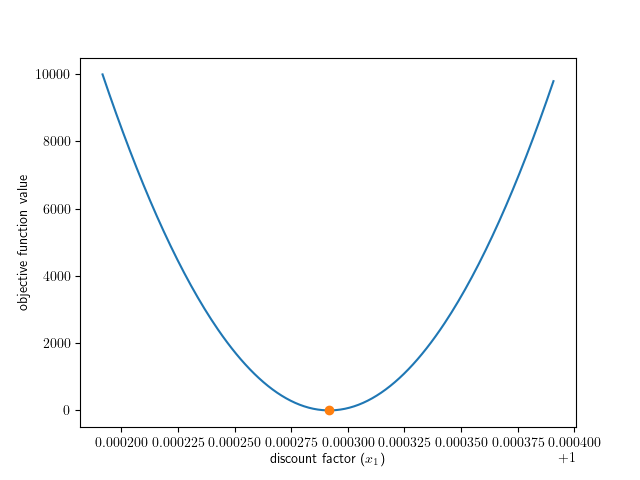
\includegraphics[width=0.45\linewidth]{obj_func.png}
  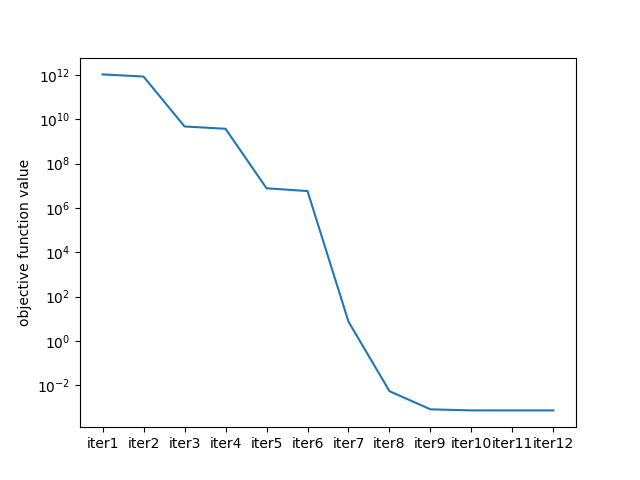
\includegraphics[width=0.45\linewidth]{obj_func_iter.png}
  \caption{On the left the objective function value as a function of discount factor $(x_{1})$,
  on the right the value of objective function at each iteration.}
\end{figure}

    \begin{Verbatim}[commandchars=\\\{\}]
{\color{incolor}In [{\color{incolor}14}]:} \PY{c+c1}{\PYZsh{} print the diagnostic of the minimization problem}
         \PY{n}{result}
\end{Verbatim}

\begin{Verbatim}[commandchars=\\\{\}]
{\color{outcolor}Out[{\color{outcolor}14}]:}       fun: 0.0007370890117814888
          hess\_inv: <34x34 LbfgsInvHessProduct with dtype=float64>
               jac: array([ 6.40061365e+05, -4.14161280e+01, -1.93984741e+01,  5.37030079e+00,
                 3.02530223e+01,  5.95243457e+01,  9.05547884e+01,  1.24363295e+02,
                 1.59125629e+02,  1.97071574e+02,  2.36973096e+02,  2.76028231e+02,
                -9.72901535e+02, -3.95831915e+02, -3.67814737e+02, -3.29982597e+02,
                -3.11447882e+02,  1.31701062e+02,  5.96919251e+02,  9.85290168e+02,
                 1.18797301e+03,  1.09656582e+03,  7.03858626e+02,  7.86777868e+01,
                -6.55082634e+02, -1.36397212e+03, -1.89121870e+02,  1.93487828e+03,
                 5.40226051e+02, -1.65947564e+02, -5.36852034e+02, -2.47750882e+03,
                -1.84414691e+02,  1.90090790e+03])
           message: b'CONVERGENCE: REL\_REDUCTION\_OF\_F\_<=\_FACTR*EPSMCH'
              nfev: 875
               nit: 12
            status: 0
           success: True
                 x: array([1.        , 1.00029175, 1.00058831, 1.00089012, 1.00116802,
                1.00147021, 1.00176786, 1.00207128, 1.00236508, 1.00266885,
                1.00297281, 1.0032578 , 1.00356124, 1.00445968, 1.00529983,
                1.00614269, 1.00693061, 1.00906201, 1.0093198 , 1.00710112,
                1.0018986 , 0.99379504, 0.9833297 , 0.97101001, 0.95723164,
                0.9426886 , 0.92772535, 0.88314869, 0.8178113 , 0.76554845,
                0.71988664, 0.64350636, 0.59281978, 0.54547324])
\end{Verbatim}
            
    \begin{Verbatim}[commandchars=\\\{\}]
{\color{incolor}In [{\color{incolor}15}]:} \PY{c+c1}{\PYZsh{} objective function value with starting point parameters}
         \PY{n}{objective\PYZus{}function}\PY{p}{(}\PY{n}{x0}\PY{p}{)} 
\end{Verbatim}

\begin{Verbatim}[commandchars=\\\{\}]
{\color{outcolor}Out[{\color{outcolor}15}]:} 1055841619695.9585
\end{Verbatim}
            
    \begin{Verbatim}[commandchars=\\\{\}]
{\color{incolor}In [{\color{incolor}16}]:} \PY{c+c1}{\PYZsh{} objective function value with final values}
         \PY{n}{objective\PYZus{}function}\PY{p}{(}\PY{n}{result}\PY{o}{.}\PY{n}{x}\PY{p}{)} 
\end{Verbatim}

\begin{Verbatim}[commandchars=\\\{\}]
{\color{outcolor}Out[{\color{outcolor}16}]:} 0.0007370890117814888
\end{Verbatim}
            
    \begin{Verbatim}[commandchars=\\\{\}]
{\color{incolor}In [{\color{incolor}17}]:} \PY{c+c1}{\PYZsh{} define the discount curve object using the }
         \PY{c+c1}{\PYZsh{} resulting discount factors (result.x)}
         \PY{n}{curve} \PY{o}{=} \PY{n}{DiscountCurve}\PY{p}{(}\PY{n}{ois\PYZus{}data}\PY{o}{.}\PY{n}{observation\PYZus{}date}\PY{p}{,} \PY{n}{pillar\PYZus{}dates}\PY{p}{,} \PY{n}{result}\PY{o}{.}\PY{n}{x}\PY{p}{)}
         
         \PY{k+kn}{from} \PY{n+nn}{datetime} \PY{k}{import} \PY{n}{date}
         \PY{n}{curve}\PY{o}{.}\PY{n}{df}\PY{p}{(}\PY{n}{date}\PY{p}{(}\PY{l+m+mi}{2059}\PY{p}{,} \PY{l+m+mi}{11}\PY{p}{,} \PY{l+m+mi}{23}\PY{p}{)}\PY{p}{)}
\end{Verbatim}

\begin{Verbatim}[commandchars=\\\{\}]
{\color{outcolor}Out[{\color{outcolor}17}]:} 0.6278698804291626
\end{Verbatim}
            
    \begin{Verbatim}[commandchars=\\\{\}]
{\color{incolor}In [{\color{incolor}18}]:} \PY{c+c1}{\PYZsh{} 50 years rate }
         \PY{k+kn}{import} \PY{n+nn}{math}
         \PY{o}{\PYZhy{}}\PY{n}{math}\PY{o}{.}\PY{n}{log}\PY{p}{(}\PY{n}{curve}\PY{o}{.}\PY{n}{df}\PY{p}{(}\PY{n}{date}\PY{p}{(}\PY{l+m+mi}{2059}\PY{p}{,} \PY{l+m+mi}{11}\PY{p}{,} \PY{l+m+mi}{23}\PY{p}{)}\PY{p}{)}\PY{p}{)} \PY{o}{/} \PY{l+m+mi}{50}
\end{Verbatim}

\begin{Verbatim}[commandchars=\\\{\}]
{\color{outcolor}Out[{\color{outcolor}18}]:} 0.009308446615020075
\end{Verbatim}
            
    \begin{Verbatim}[commandchars=\\\{\}]
{\color{incolor}In [{\color{incolor}19}]:} \PY{n+nb}{list}\PY{p}{(}\PY{n}{result}\PY{o}{.}\PY{n}{x}\PY{p}{)}
\end{Verbatim}

\begin{Verbatim}[commandchars=\\\{\}]
{\color{outcolor}Out[{\color{outcolor}19}]:} [1.0,
          1.0002917467402102,
          1.000588313127234,
          1.0008901199538132,
          1.0011680243827574,
          1.0014702089411056,
          1.0017678648937525,
          1.0020712764009663,
          1.0023650754871605,
          1.0026688489207223,
          1.0029728065322203,
          1.0032577961650246,
          1.003561243417754,
          1.004459676763001,
          1.0052998330195508,
          1.0061426892577996,
          1.006930607427503,
          1.009062012124004,
          1.0093198010277291,
          1.0071011202466504,
          1.00189860229147,
          0.9937950392360159,
          0.9833296977458316,
          0.9710100057905164,
          0.9572316430523317,
          0.9426886049809743,
          0.9277253536938298,
          0.8831486876894581,
          0.817811304643707,
          0.7655484543652669,
          0.7198866407284839,
          0.643506361425598,
          0.5928197767210946,
          0.5454732370629979]
\end{Verbatim}
            
    \begin{Verbatim}[commandchars=\\\{\}]
{\color{incolor}In [{\color{incolor}20}]:} \PY{n}{pillar\PYZus{}dates}
\end{Verbatim}

\begin{Verbatim}[commandchars=\\\{\}]
{\color{outcolor}Out[{\color{outcolor}20}]:} [datetime.date(2016, 11, 23),
          datetime.date(2016, 12, 23),
          datetime.date(2017, 1, 23),
          datetime.date(2017, 2, 23),
          datetime.date(2017, 3, 23),
          datetime.date(2017, 4, 23),
          datetime.date(2017, 5, 23),
          datetime.date(2017, 6, 23),
          datetime.date(2017, 7, 23),
          datetime.date(2017, 8, 23),
          datetime.date(2017, 9, 23),
          datetime.date(2017, 10, 23),
          datetime.date(2017, 11, 23),
          datetime.date(2018, 2, 23),
          datetime.date(2018, 5, 23),
          datetime.date(2018, 8, 23),
          datetime.date(2018, 11, 23),
          datetime.date(2019, 11, 23),
          datetime.date(2020, 11, 23),
          datetime.date(2021, 11, 23),
          datetime.date(2022, 11, 23),
          datetime.date(2023, 11, 23),
          datetime.date(2024, 11, 23),
          datetime.date(2025, 11, 23),
          datetime.date(2026, 11, 23),
          datetime.date(2027, 11, 23),
          datetime.date(2028, 11, 23),
          datetime.date(2031, 11, 23),
          datetime.date(2036, 11, 23),
          datetime.date(2041, 11, 23),
          datetime.date(2046, 11, 23),
          datetime.date(2056, 11, 23),
          datetime.date(2066, 11, 23),
          datetime.date(2076, 11, 23)]
\end{Verbatim}
            
    \hypertarget{exercises}{%
\subsection{Exercises}\label{exercises}}

\hypertarget{exercise-5.2}{%
\subsubsection{Exercise 5.2}\label{exercise-5.2}}

Take the \texttt{OvernightIndexSwap} class from the lesson and add a new
method called fair\_value\_strike which takes a discount curve object
and returns the fixed rate which would make the OIS have zero NPV.

\emph{Hints}:
\begin{itemize}
\item first take the formulas for the NPV of the fixed leg and
the NPV of the floating leg, put one equal to the other and solve for
$K$;
\item then implement that in Python.
\end{itemize}

\hypertarget{exercise-5.3}{%
\subsubsection{Exercise 5.3}\label{exercise-5.3}}

Take the \texttt{OvernightIndexSwap} class, add it to
\texttt{finmarkets.py} and try importing and using it.


    % Add a bibliography block to the postdoc
    
    
    
    \end{document}
